\chapter{Workloads}
\label{section:workloads}

%%%%%%%%%%%%%%%%%%%%%%%%%%%%%%%%%%%%%%%%%%%%%%%%%%%%%%%%%%%%%%%%%%%%%%%%%%%%%%
%%%%%%%%%%%%%%%%%%%%%%%%%%%%%%%%%%%%%%%%%%%%%%%%%%%%%%%%%%%%%%%%%%%%%%%%%%%%%%
%%%%%%%%%%%%%%%%%%%%%%%%%%%%%%%%%%%%%%%%%%%%%%%%%%%%%%%%%%%%%%%%%%%%%%%%%%%%%%

\section{Query Description Format}
\label{sub:queries_structure}
Queries are described in natural language using a well-defined structure that consists of three sections:
\textit{description}, a concise textual description of the query;
\textit{parameters}, a list of input parameters and their types;
and \textit{results}, a list of expected results and their types.
The syntax used in \textit{parameters} and \textit{results} sections is as follows:

\begin{itemize}
    \item \textbf{Entity}: entity type in the dataset.\\
        One word, possibly constructed by appending multiple words together, starting with uppercase character and following the camel case notation,
        \eg \texttt{TagClass} represents an entity of type ``TagClass''.
    \item \textbf{Relationship}: relationship type in the dataset.\\
        One word, possibly constructed by appending multiple words together, starting with lowercase character and following the camel case notation,
        and surrounded by arrow to communicate direction,
        \eg \mbox{\texttt{-worksAt->}} represents a directed relationship of type ``worksAt''.
    \item \textbf{Attribute}: attribute of an entity or relationship in the dataset.\\
        One word, possibly constructed by appending multiple words together, starting with lowercase character and following the camel case notation,
        and prefixed by a ``.'' to dereference the entity/relationship,
        \eg \texttt{Person.firstName} refers to ``firstName'' attribute on the ``Person'' entity,
        and \mbox{\texttt{-studyAt->.classYear}} refers to ``classYear'' attribute on the ``studyAt'' relationship.
    \item \textbf{Unordered Set}: an unordered collection of distinct elements.\\
        Surrounded by \{ and \} braces, with the element type between them,
        \eg \texttt{\{String\}} refers to a set of strings.
    \item \textbf{Ordered List}: an ordered collection where duplicate elements are allowed.\\
        Surrounded by [ and ] braces, with the element type between them,
        \eg \texttt{[String]} refers to a list of strings.
    \item \textbf{Ordered Tuple}: a fixed length, fixed order list of elements, where elements at each position of the tuple have predefined, possibly different, types. \\
        Surrounded by < and > braces, with the element types between them in a specific order
        \eg \texttt{<String, Boolean>} refers to a 2-tuple containing a string value in the first element and a boolean value in the second,
        and \texttt{[<String, Boolean>]} is an ordered list of those 2-tuples.
\end{itemize}

\paragraph{Categorization of results.} Results are categorized according to their source of origin:

\begin{itemize}
	\item \textbf{Raw} (\texttt{R}), if the result is returned with an unmodified value and type.
	\item \textbf{Calculated} (\texttt{C}), if the result is calculated from other values and conditions.
	\item \textbf{Aggregated} (\texttt{A}), if the result is an aggregated value, \eg a count or a sum of another value. If a result is both calculated and aggregated (\eg $\mathsf{count(x) + count(y)}$ or $\mathsf{avg(x + y)}$), it is considered an aggregated result.
	\item \textbf{Meta} (\texttt{M}), if the result is based on type information, \eg the type of the node.
\end{itemize}


%%%%%%%%%%%%%%%%%%%%%%%%%%%%%%%%%%%%%%%%%%%%%%%%%%%%%%%%%%%%%%%%%%%%%%%%%%%%%%
%%%%%%%%%%%%%%%%%%%%%%%%%%%%%%%%%%%%%%%%%%%%%%%%%%%%%%%%%%%%%%%%%%%%%%%%%%%%%%
%%%%%%%%%%%%%%%%%%%%%%%%%%%%%%%%%%%%%%%%%%%%%%%%%%%%%%%%%%%%%%%%%%%%%%%%%%%%%%

\section{Conventions for Query Definitions}

\paragraph{Interval notations.} Closed interval boundaries are denoted with 
\texttt{[} 
and \texttt{]}, while open interval boundaries are denoted with \texttt{(} and 
\texttt{)}. For example, \texttt{[0, 1)} denoted an interval between 0 and 1, 
closed on the left and open on the right.

\paragraph{Comparing Date and DateTime values.}

Some query specifications (\eg \queryRefCard{bi-read-01}{BI}{1}, 
\queryRefCard{bi-read-02}{BI}{2}, etc.) require implementations to compare a 
$\mathsf{DateTime}$ value with a $\mathsf{Date}$ value. In these cases, the 
$\mathsf{Date}$ value should be implicitly converted $\mathsf{DateTime}$ value 
with a time of 00:00:00.000+0000 (\ie with the timezone of GMT).

\paragraph{Matching semantics.}

Unless noted otherwise, the specification uses \emph{homomorphic} matching 
semantics~\cite{Angles:2017:FMQ:3145473.3104031}, \ie both nodes and edges can 
occur multiple times in a match. Note that for variable length path, duplicate 
edges are not allowed.

\paragraph{Aggregation semantics.}

The \lstinline{count} aggregation always requires the query to determine the number of \emph{distinct} elements (nodes or edges). For example, this can be achieved in the Cypher, SPARQL and SQL query languages with the \lstinline[language=sql]{count(DISTINCT ...)} construct.

\paragraph{Graph patterns.}

To illustrate queries, we use graph patterns such as \autoref{fig:example-graph-pattern} with the following notation:

\begin{figure}[ht]
	\begin{center}
		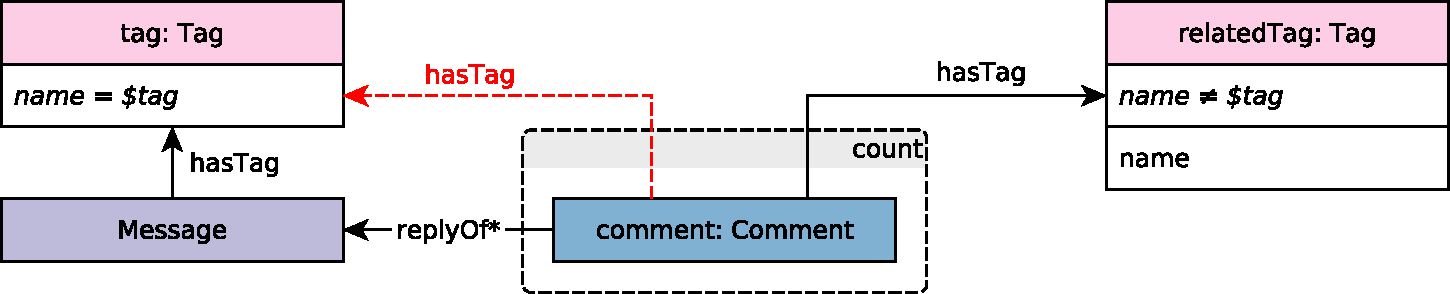
\includegraphics[scale=\patternscale,margin=0cm .2cm]{patterns/bi-read-08}
		\caption{Example graph pattern.}
		\label{fig:example-graph-pattern}
	\end{center}
\end{figure}

\begin{itemize}
	\item Nodes are marked as $\mathsf{entityName: EntityType}$ (camel case 
	notation for both, starting with a lowercase character for the first and an 
	uppercase character for the second). If the $\mathsf{entityName}$ is not used 
	in the query results, aggregations or calculations, and not referenced in the 
	query specification, the $\mathsf{entityName}$ can be omitted.
	\item Positive conditions for edges are denoted with solid lines.
	\item Negative conditions for edges, \ie edges that are not allowed in the graph, are denoted with \textcolor{red}{\dashuline{dashed red}} lines.
	\item Edges without direction imply that there must be an edge in \emph{at least one of the directions}.
	\item Filtering conditions are typeset in \textit{italic}, \eg $\mathit{id} = 
	\mathit{\textdollar tag}$.
	\item Attributes that should be returned are denoted in sans-serif font, \eg $\mathsf{name}$.
	\item Variable length paths, \ie edges that can be traversed multiple times 
	are denoted with $*\mathsf{min}...\mathsf{max}$, \eg $\mathsf{replyOf}*$ or 
	$\mathsf{knows*1 \ldots 2}$. By default, the value of $\mathsf{min}$ is 1, 
	and the value of $\mathsf{max}$ is unlimited.
	\item Aggregations are shown in dashed boxes with the type of aggregation ($\mathsf{count}$, $\mathsf{sum}$, $\mathsf{avg}$, etc.) in the upper right corner.
\end{itemize}

\newcommand{\tuple}[1]{\langle #1 \rangle}

\paragraph{Keywords.} The pattern notation uses a small set of keywords:

\begin{itemize}
	\item $\mathsf{UNWIND}$ unnests a list, \ie produces a set of one-tuples. For 
	example, $\mathsf{UNWIND} [1, 2, 3]$ results in $ \{ \tuple{1}, \tuple{2}, 
	\tuple{3} \} $.
	\item Aggregation operations: \lstinline{count}, \lstinline{avg}. % \lstinline{sum} - sum is not used in the figures as we always sum some derived value
	\item Functions:
	\begin{itemize}
		\item \lstinline{floor(x)} (returns $\lfloor x \rfloor$),
		\item \lstinline{year(date)} (extracts the year from a given date),
		\item \lstinline{month(date)} (extracts the month from a given date).
	\end{itemize}
\end{itemize}

\paragraph{Resolving ambiguity.} Note that if the textual description and the graph pattern are different for a particular query (either due to an error or the lack of sophistication in the graphical syntax), \emph{the textual description takes precedence}.

%%%%%%%%%%%%%%%%%%%%%%%%%%%%%%%%%%%%%%%%%%%%%%%%%%%%%%%%%%%%%%%%%%%%%%%%%%%%%%
%%%%%%%%%%%%%%%%%%%%%%%%%%%%%%%%%%%%%%%%%%%%%%%%%%%%%%%%%%%%%%%%%%%%%%%%%%%%%%
%%%%%%%%%%%%%%%%%%%%%%%%%%%%%%%%%%%%%%%%%%%%%%%%%%%%%%%%%%%%%%%%%%%%%%%%%%%%%%

\section{Substitution Parameters}

Together with the dataset, \datagen produces a set of parameters per
query type. Parameter generation is designed in such a way that for each query
type, all of the generated parameters yield similar runtime behaviour of that
query.

Specifically, the selection of parameters for a query template guarantees the following properties of the resulting queries:
\begin{enumerate}
\item[P1:] the query runtime has a bounded variance: the average runtime corresponds to the behavior of the majority of the queries
\item[P2:] the runtime distribution is stable: different samples of (\eg 10) parameter bindings used in different query streams result in an identical runtime distribution across streams
\item[P3:] the optimal logical plan (optimal operator order) of the queries is the same: this ensures that a specific query template tests the system's behavior under the well-chosen technical difficulty (\eg handling voluminous joins or proper cardinality estimation for subqueries, \etc)
\end{enumerate}


As a result, the amount of data that the query touches is roughly the
same for every parameter binding, assuming that the query optimizer figures out a
reasonable execution plan for the query. This is done to avoid bindings that
cause unexpectedly long or short runtimes of queries, or even result in a
completely different optimal execution plan. Such effects could arise due to
the data skew and correlations between values in the generated dataset.

In order to get the parameter bindings for each of the queries, we have designed a \textit{Parameter Curation} procedure that works in two stages:

\begin{enumerate}
\item for each query template for all possible parameter bindings, we determine the size of intermediate results in the {\em intended} query plan. Intermediate result size heavily influences the runtime of a query, so two queries with the same operator tree and similar intermediate result sizes at every level of this operator tree are expected to have similar runtimes. This analysis is effectively a side effect of data generation, that is we keep all the necessary counts (number of friends per user, number of posts of friends \etc) as we create the dataset.
\item then, a greedy algorithm selects (``curates'') those parameters with similar intermediate result counts from the domain of all the parameters.
\end{enumerate}

Parameter bindings are stored in the \texttt{substitution\_parameters} folder
inside the data generator directory. Each query gets its bindings in a separate
file. Every line of a parameter file is a JSON-formatted collection of
key-value pairs (name of the parameter and its value). For example, the Query 1
parameter bindings are stored in file \texttt{query\_1\_param.txt}, and one of
its lines may look like this:

\vspace{-6mm}
$$
\{\text{"PersonID"}: 1, \text{"Name"}: \text{"Lei"}, \text{"PersonURI"}: \text{"http://www.ldbc.eu/ldbc\_socialnet/1.0/data/pers1"}\}
$$

Depending on implementation, the SUT may refer to persons either by IDs
(relational and graph databases) or URIs (RDF systems), so we provide both
values for the Person parameter.  Finally, parameters for short reads are taken
from those in complex reads and updates.


%%%%%%%%%%%%%%%%%%%%%%%%%%%%%%%%%%%%%%%%%%%%%%%%%%%%%%%%%%%%%%%%%%%%%%%%%%%%%%
%%%%%%%%%%%%%%%%%%%%%%%%%%%%%%%%%%%%%%%%%%%%%%%%%%%%%%%%%%%%%%%%%%%%%%%%%%%%%%
%%%%%%%%%%%%%%%%%%%%%%%%%%%%%%%%%%%%%%%%%%%%%%%%%%%%%%%%%%%%%%%%%%%%%%%%%%%%%%

\section{Load Definition}

\ldbcsnb Test Driver is in charge of the execution of the Interactive Workload.
At the beginning of the execution, the Test Driver creates a query mix by
assigning to each query instance, a query issue time and a set of parameters
taken from the generated substitution parameter set described above.  

Query issue times have to be carefully assigned.  Although substitution
parameters are chosen in such a way that queries of the same type take similar
time, not all query types have the same complexity and touch the same amount of
data, which causes them to scale differently for the different scale factors.
Therefore, if all query instances, regardless of their type, are issued
at the same rate, those more complex queries will dominate the execution's
result, making faster query types purposeless. To avoid this situation, each
query type is executed at a different rate. The way the execution rate is decided,
also depends on the nature of the query: complex read, short read or update.

Update queries' issue times are taken from the update streams generated by the
data generator. These are the times where the actual event happened during the
simulation of the social network. Complex reads' times are expressed in terms
of update operations. For each complex read query type, a frequency value is
assigned which specifies the relation between the number of updates performed
per complex read.  Table~\ref{table:freqs} shows the frequencies assigned to
each query type for SF1. The frequencies of the different scale factors can be
found in Appendix~\ref{appendix:scale_factors}.

\begin{table}[H]
\centering
    \begin{tabular}{|c|c|c|c|}
    \hline
    Query Type & freq & Query Type & freq \\ 
    \hline
    \hline
    Query 1 & 26 & Query 8 & 45 \\ 
    \hline       
    Query 2 & 37 & Query 9 & 157 \\  
    \hline        
    Query 3 & 69 & Query 10 & 30 \\ 
    \hline        
    Query 4 & 36 & Query 11 & 16 \\ 
    \hline        
    Query 5 & 57 & Query 12 & 44 \\ 
    \hline        
    Query 6 & 129 & Query 13 & 19 \\  
    \hline        
    Query 7 & 87 & Query 14 & 49 \\ 
    \hline
    \end{tabular}
    \caption{Frequencies for each query type for SF1.}
    \label{table:freqs}
\end{table}

Finally, short reads are inserted in order to balance the ratio between reads
and writes, and to simulate the behavior of a real user of the social network.
For each complex read instance, a sequence of short reads is planned. There are two
types of short read sequences: Person centric and Message centric. Depending on
the type of the complex read, one of them is chosen. Each sequence consists of
a set of short reads which are issued in a row. The issue time assigned to each
short read in the sequence is determined at run time, and is based on the
completion time of the complex read it depends on. 
The substitution parameters for short reads are taken from the results of previously
executed complex reads and short reads.
Once a short read sequence is issued (and provided that sufficient substitution parameters 
exist), there is a probability that another short read  sequence is issued. 
This probability decreases for each new sequence issued. 
Since the same random number generator seed is used across
executions, the workload is deterministic.


The specified frequencies, implicitly define the query ratios between queries
of different types, as well as a default target throughput. However the Test
Sponsor may specify a different target throughput to test,  by ``squeezing''
together or ``stretching'' apart the queries of the workload. This is
achieved  by means of the ``Time Compression Ratio'' that is multiplied by the
frequencies (see \autoref{table:freqs}).  Therefore, different
throughputs can be tested while maintaining the relative ratios between the
different query types.
